\question{Câu 13}

Cho mạch điện như hình 13a, OPAMP được cấp nguồn  có $V_{OH} = 3.3\,\textsf{V}$, $V_{OL} = -3\,\textsf{V}$. Các điện trở được chọn $R_{1} = 2\,\textsf{k}\Omega$, $R_{2} = 3\,\textsf{k}\Omega$, $R_{3} = 4\,\textsf{k}\Omega$ và $R_{4} = 6\,\textsf{k}\Omega$. Cho dạng sóng $V_{i}(t)$ như hình 13b.

 \begin{minipage}{.5\linewidth}
	\begin{figure}[H]
		\centering
		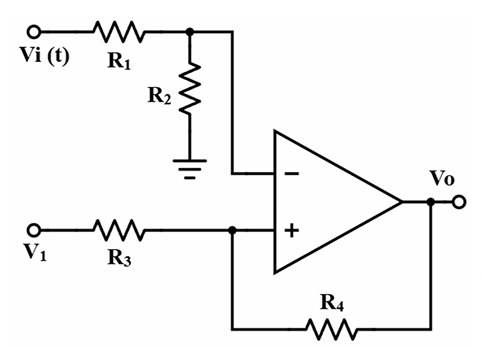
\includegraphics[width=.9\linewidth]{./my-chapters/my-images/Question13/debai_13a.png}
		\caption*{Hình 13a.}
	\end{figure}
\end{minipage}
\begin{minipage}{.5\linewidth}
	\begin{figure}[H]
		\centering
		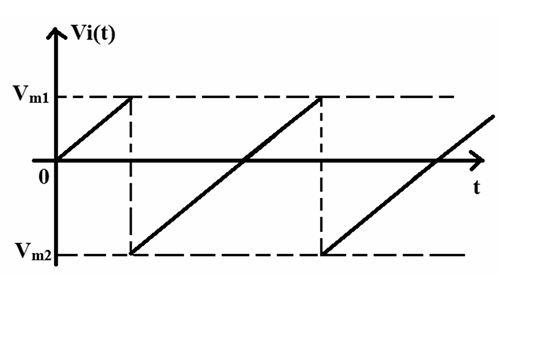
\includegraphics[width=\linewidth]{./my-chapters/my-images/Question13/debai_13b.png}
		\caption*{Hình 13b.}
	\end{figure}
\end{minipage}

 \answer{a}{Vẽ dạng sóng ngõ ra $V_{o}$ trong trường hợp $V_{1} = 2\,\textsf{V}$, $V_{m1} = 2\,\textsf{V}$, $V_{m2} = -3\,\textsf{V}$.}
 
 Ta có: $V_{-} = \dfrac{R_{2}}{R_{1} + R_{2}} V_{in} \rightarrow V_{-} = \dfrac{3}{5} V_{in}$
 \[
 \dfrac{V_{in}-V_{+}}{R_{1}} = \dfrac{V_{+}}{R_{3}} + \dfrac{V_{+}-V_{o}}{R_{2}}
 \]
 \[
 \rightarrow V_{+} = R_{3}//R_{4}\left(\dfrac{V_{1}}{R_{3}} +\dfrac{V_{o}}{R_{4}} \right) \\[6pt]
 \rightarrow  V_{+} = \dfrac{3V_{1}}{5}\ + \dfrac{2V_{o}}{5}
 \]
 
 Khi $V_{o}$ đang ở mức thấp để chuyển sang mức cao  $\rightarrow V_{+} > V_{-}$
 \[
 \rightarrow \dfrac{3V_{1}}{5}\ + \dfrac{2V_{OL}}{5} > \dfrac{3}{5} V_{in} \rightarrow V_{in} < 0 \,\textsf{V}
 \]
 
 Khi $V_{o}$ đang ở mức cao để chuyển sang mức thấp  $\rightarrow V_{+} < V_{-}$
 \[
 \rightarrow \dfrac{3V_{1}}{5}\ + \dfrac{2V_{OH}}{5} < \dfrac{3}{5} V_{in} \rightarrow V_{in} > 4.2 \,\textsf{V}
 \]
 
 \begin{figure}[H]
 	\centering
 	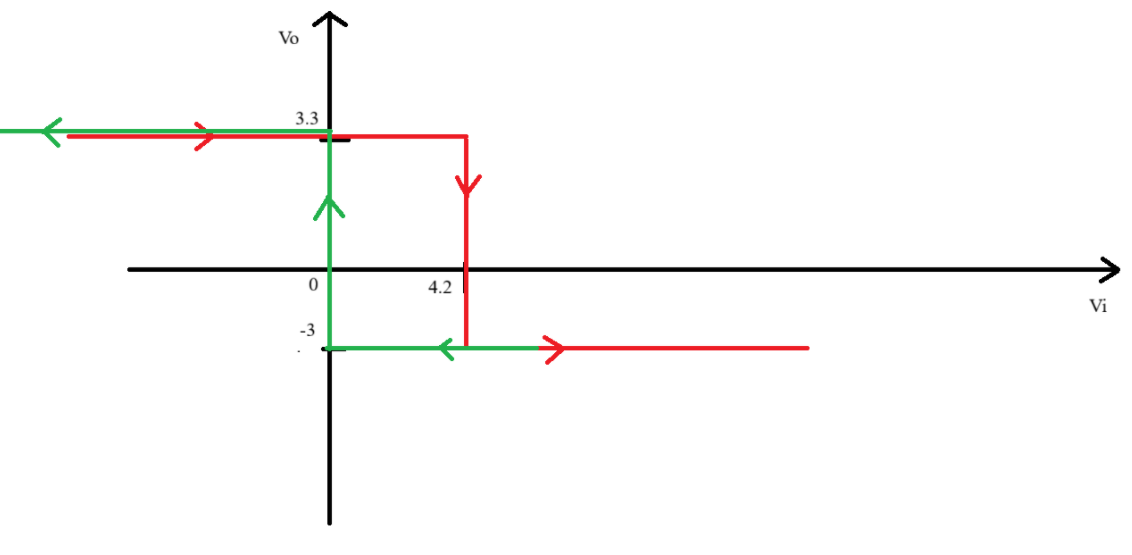
\includegraphics[width=.9\linewidth]{./my-chapters/my-images/Question13/C13_Hình1.png}
 	\caption{Đồ thị $V_{o}$ theo $V_{i}$.}
 \end{figure}
 
 Với $V_{m1} = 2 \,\textsf{V}$, $V_{m2} = -3\,\textsf{V}$
 
 Tính từ thời gian $t = 0$, $V_{i} =0\,\textsf{V}$ cho đến $2\,\textsf{V}$ ngõ ra có thể là $V_{OH}$ và $V_{OL}$ tùy thuộc vào giá trị độ lệch $V_{os}$ của $V_{+}$ và $V_{-}$. Khi $V_{i} < 0 \rightarrow V_{o}$ luôn ở mức cao từ thời điểm đó trở đi $\Rightarrow V_{o} = V_{OH} = 3.3\,\textsf{V}$.
 
 \begin{figure}[H]
 	\centering
 	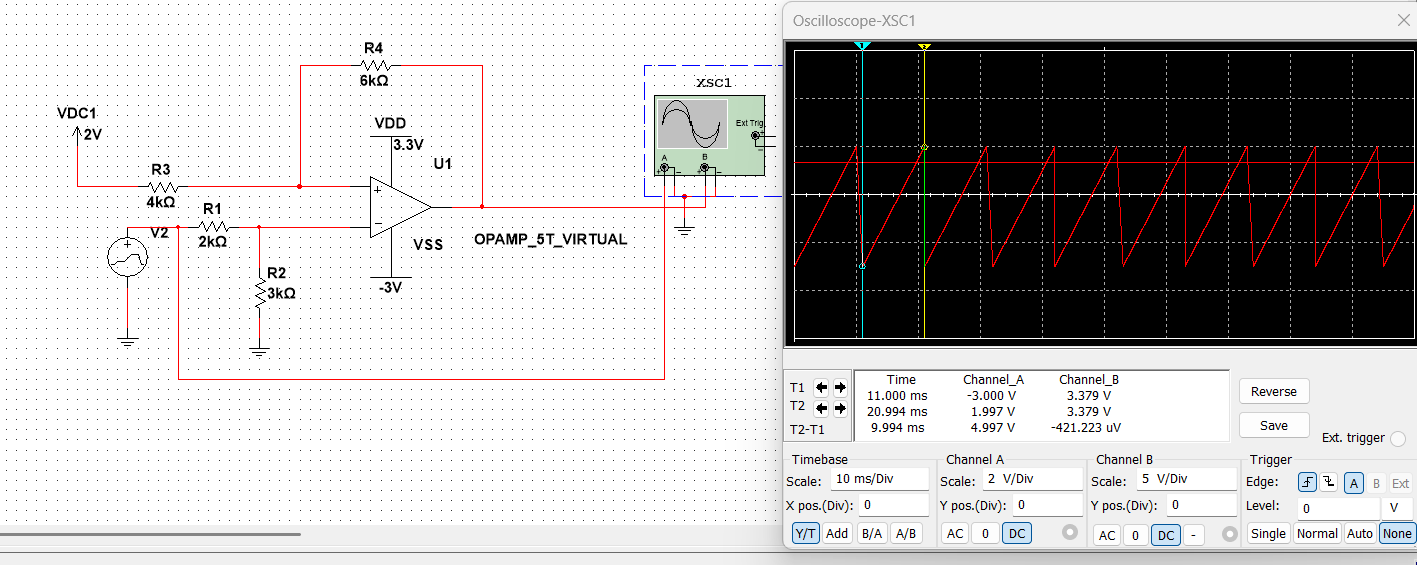
\includegraphics[width=.9\linewidth]{./my-chapters/my-images/Question13/C13_Hình2.png}
 	\caption{Mô phỏng Multisim.}
 \end{figure}
 
  \answer{b}{Vẽ dạng sóng ngõ ra $V_{o}$ trong trường hợp $V_{1} = 4\,\textsf{V}$, $V_{m1} = 1\,\textsf{V}$, $V_{m2} = -3\,\textsf{V}$.}
  
  Khi $V_{o}$ đang ở mức thấp để chuyển sang mức cao $\rightarrow V_{+} > V_{-} $
  \[\rightarrow \dfrac{3V_{1}}{5} +\dfrac{2V_{OL}}{5} > \dfrac{3}{5} \rightarrow V_{in} < 2 \,\textsf{V}\]
  Khi $V_{o}$ đang ở mức cao để chuyển sang mức thấp $\rightarrow V_{+} < V_{-} $
  \[\rightarrow \dfrac{3V_{in}}{5} +\dfrac{2V_{OH}}{5} < \dfrac{3}{5} \rightarrow V_{in} > 6.2 \,\textsf{V}\]
  
  \begin{figure}[H]
  	\centering
  	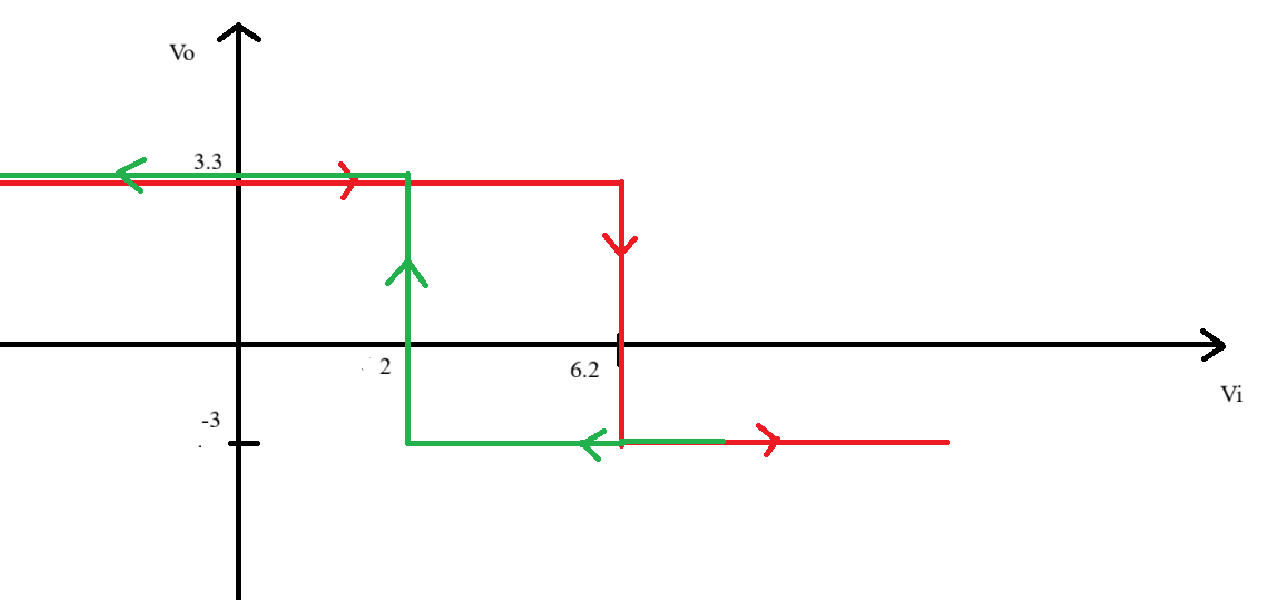
\includegraphics[width=.9\linewidth]{./my-chapters/my-images/Question13/C13_Hình3.png}
  	\caption{Đồ thị $V_{o}$ theo $V_{i}$.}
  \end{figure}
  
  Với $V_{m1} = 1\,\textsf{V}$, $V_{m2} = -3\,\textsf{V}$, $V_{o}$ luôn ở mức thấp $\rightarrow V_{o} = V_{OH} = 3.3\,\textsf{V}$
  
  \begin{figure}[H]
  	\centering
  	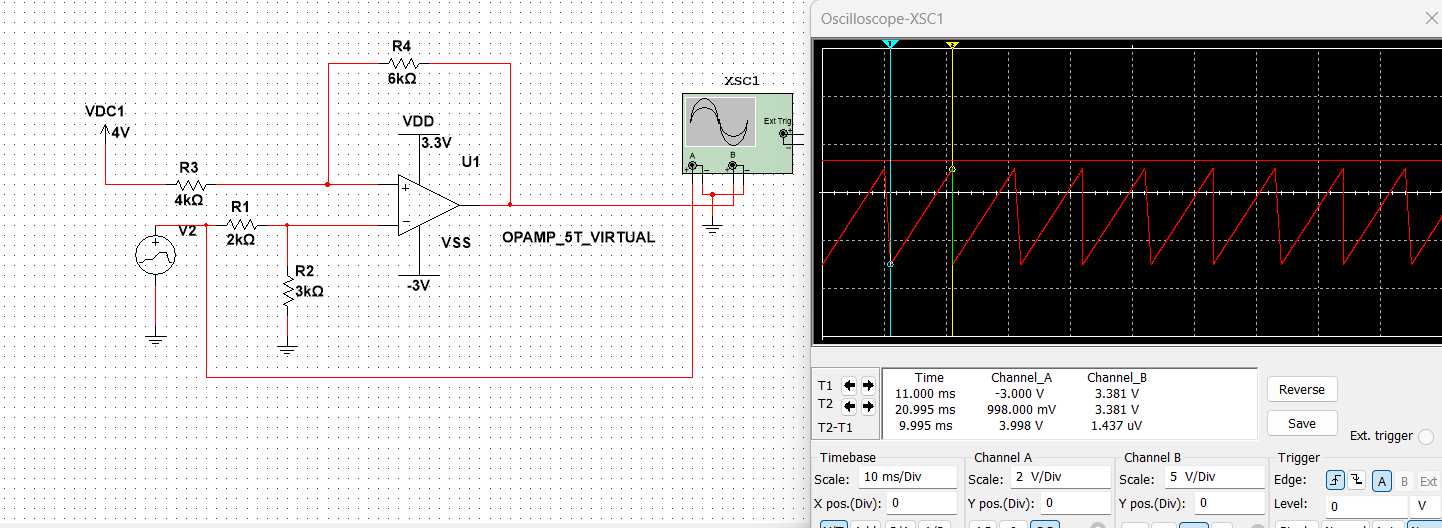
\includegraphics[width=.8\linewidth]{./my-chapters/my-images/Question13/C13_Hình4.png}
  	\caption{Mô phỏng Multisim.}
  \end{figure}